\section{Modèle cinématique}

Afin de déterminer un modèle pour l'ensemble du mouvement de notre système (notre essaim de deux robots), on s'intéresse d'abord au mouvement d'un seul robot. 

Le robot Pololu Zumo est une petite plate-forme robotique à chenilles de moins de 10 cm de côté et fonctionne avec une variété de micro-moteurs à engrenages métalliques pour permettre une combinaison personnalisable de couple et de vitesse. \cite{pololu-url}. Les deux chenilles contribuent au mouvement du robot et, en même temps, imposent des contraintes au mouvement du robot. 

Ce type de robot est appelé \textit{« differential-drive »}, signifiant que le mouvement est basé sur deux roues (ou chenilles dans notre cas) entraînées séparément et placées de chaque côté du corps du robot. Il peut ainsi changer de direction en faisant varier le taux de rotation relatif de ses roues et ne nécessite donc pas de mouvement de direction supplémentaire. Si les deux roues sont entraînées dans le même sens et à la même vitesse, le robot se déplace en ligne droite. Si les deux roues sont entraînées à la même vitesse dans des directions opposées, le robot tournera autour du point central de l'axe. \cite{Differential-drive-wikipedia-url}

\subsection{Representing robot position - Représentation de la position du robot}

Nous modélisons le robot comme un corps rigide à chenilles, opérant sur un plan horizontal, homogène et faiblement cohésif. 

\begin{figure}[h!]
    \centering
    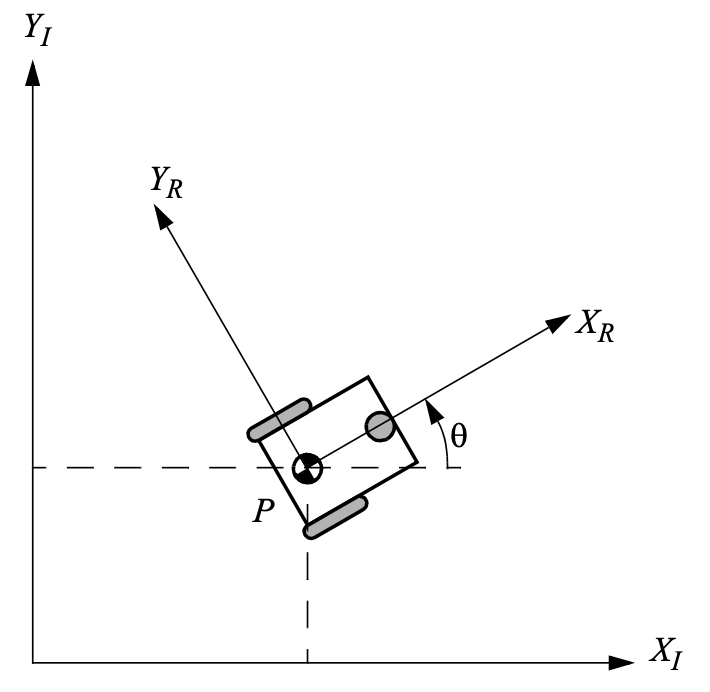
\includegraphics[scale=0.5]{img/3_kinematic_model/reference_frames.png}
    \caption{Le référentiel global et le référentiel local du robot.}
    \label{fig:reference_frames}
\end{figure}

Les axes $\hat{X}_I$ et $\hat{Y}_I$ définissent une base inertielle arbitraire sur le plan en tant que cadre de référence global à partir d'une origine $O:\{ \hat{X}_I, \hat{Y}_I \}$. Pour spécifier la position du robot, nous choisissons un point $P$ sur le châssis du robot, centré entre les deux roues motrices, comme point de référence de sa position. La base $\{\hat{X}_R, \hat{Y}_I \}$ définit deux axes relatifs à $P$ qui constituent donc le cadre de référence local du robot. La position de $P$ dans le cadre de référence global est spécifiée par les coordonnées $x$ et $y$, et la différence angulaire entre les cadres de référence global et local est donnée par $\theta$. Nous pouvons décrire la position du robot comme un vecteur avec ces trois éléments, où l'indice $I$ indique que la base est le cadre de référence global :

\begin{equation}
    \xi = \left [
\begin{array}{l}
     x  \\
     y  \\
     \theta
\end{array}
    \right ]
    \label{eq:position}
\end{equation}

Afin de spécifier la position du robot sur le plan, nous établissons une relation entre le référentiel global du plan et le référentiel local du robot, la \textit{matrice de rotation orthogonale}:
\begin{equation}
    R(\theta) = \left [
    \begin{array}{ccc}
        \cos(\theta) & \sin(\theta) & 0 \\
        -\sin(\theta) & \cos(\theta) & 0 \\
        0 & 0 & 1 \\
    \end{array}
    \right ]
\end{equation}

Cette matrice peut être utilisée pour convertir le mouvement dans le cadre de référence global en mouvement dans le cadre de référence local. Cette opération est dénotée par $\dot{\xi_R} = R(\theta) \cdot \dot{\xi_I}$.

\subsection{Forward kinematic models - Modèle cinématique}

Le robot possède deux roues, chacune de diamètre $r$. Étant donné un point $P$ situé entre les deux roues motrices, chaque roue est à une distance $l$ de $P$.

Étant donné $r$, $l$, $\theta$ et la vitesse de rotation de chaque roue, $\dot{\varphi_1}$ et $\dot{\varphi_2}$, un modèle cinématique peut prédire la vitesse globale du robot dans le cadre de référence global: 

\begin{equation}
    \dot{\xi_I} = \left [\begin{array}{c}
        \dot{x} \\
        \dot{y} \\
        \dot{\theta}
        \end{array} \right ]= f \left ( l, r, \theta, \dot{\varphi_1}, \dot{\varphi_2} \right )
\end{equation}

\subsection{Wheel kinematic constraints - Fixed standard wheel}

\subsection{Robot kinematic constraints}

\subsection{Path and trajectory considerations}

$\\
x_1=\frac{2x_T+d_x}{2}\\
x_2=\frac{2x_T-d_x}{2}\\
y_1=\frac{2y_T+d_y}{2}\\
y_2=\frac{2y_T-d_y}{2}\\
\delta\theta=\frac{(v_d-v_g)\delta t}{L}\\
v_x=\dot{x}=\frac{v_g_x+v_d_x}{2}\\
v_y=\dot{y}=\frac{v_g_y+v_d_y}{2}\\
$